\documentclass[12,french]{report}
\usepackage{geometry}
\geometry{vmargin=3cm, hmargin=3cm}
\usepackage[T1]{fontenc}
\usepackage[utf8]{inputenc}
\usepackage[french]{babel}
\usepackage{graphicx}
\usepackage{amsmath}
\usepackage{amssymb}
\usepackage{sectsty}
\usepackage{authblk}
\usepackage{algpseudocode}
\usepackage{algorithm}
\usepackage{xspace}
\usepackage{mathtools}
\usepackage{mathrsfs}
\usepackage{enumitem}
\usepackage{titlesec}
\usepackage{hyperref}
\usepackage{xcolor}
\usepackage[justification=centering]{caption}
\usepackage{float}
\usepackage{tabto}
\usepackage{algorithm}
\usepackage{algpseudocode}
\usepackage{ulem}

\usepackage{listings}
\usepackage{cleveref}

\renewcommand{\lstlistingname}{Code}
%\renewcommand{\figurename}{Fig.}
\renewcommand\listalgorithmname{Liste des algorithmes}


\lstdefinestyle{chstyle}{%
backgroundcolor=\color{gray!12},
basicstyle=\ttfamily\small,
showstringspaces=false,
numbers=left}

%\AddThinSpaceBeforeFootnotes
%\FrenchFootnotes

\titleformat{\chapter}[hang]{\bf\Huge}{\thechapter.}{2pc}{}
\titlespacing*{\chapter}{10pt}{0pt}{40pt}[0pt]
\newcommand{\HRule}{\rule{\linewidth}{0.5mm}}

\providecommand{\keywords}[1]{\textbf{\textit{Keywords:}} #1}
\bibliographystyle{apalike}

\usepackage{hyperref}

\begin{document}
\hypersetup{pdfborder=0 0 0}

\begin{titlepage}

\begin{center}
	\vspace*{\stretch{1}}
	\textsc{{\LARGE Institut national des sciences appliquées de Rouen} \\ 			\vspace{6mm} {\Large INSA de Rouen}} \\
	\vspace{5mm}
	
\includegraphics[width=0.4\textwidth]{./Images/insa}\\[1.0 cm]

	\textsc{\Large Projet Info GM4 - Vague 1}\\[0.6cm]

	% Title
	\HRule \\[0.5cm]
	{ \Huge \bfseries Algorithme Min-Max}\\[0.2cm]
	\HRule \\[0.75cm]

	
\includegraphics[width=0.7\textwidth]{./Images/Page_de_garde}\\[0.9 cm]

	% Author and supervisor
	\begin{minipage}{0.4\textwidth}
		\begin{flushleft} \large
			\emph{Auteurs:}\\
			Thibaut \textsc{André-Gallis} \\
			{\small\href{mailto:thibaut.andregallis@insa-rouen.fr}{thibaut.andregallis@insa-rouen.fr}} \\
			Kévin \textsc{Gatel} \\
			{\small\href{mailto:kevin.gatel@insa-rouen.fr}{kevin.gatel@insa-				rouen.fr}}\\
			Chloé \textsc{Mechelinck} \\
			{\small\href{mailto:chloe.mechelinck@insa-rouen.fr}{chloe.mechelinck@insa-rouen.fr}}
		\end{flushleft}
	\end{minipage}
	\begin{minipage}{0.4\textwidth}
		\begin{flushright} \large
			\emph{Enseignants:} \\
			Nathalie \textsc{Chaignaud} \\
			{\small\href{mailto:nathalie.chaignaud@insa-rouen.fr}								{nathalie.chaignaud@insa-rouen.fr}}\\
		\end{flushright}
	\end{minipage}
	\vspace*{\stretch{1}}

	\vfill
	{\large 04 Janvier 2022}
\end{center}
\end{titlepage}

\tableofcontents

\renewcommand{\chaptername}{}

\chapter*{Introduction}

Le projet semestriel que nous avons choisi est de créer une intelligence artificielle (IA) grâce à l'algorithme Min-Max. 


Le but du projet est de mettre en œuvre les compétences acquises en programmation orientée objet et de nous ouvrir à un domaine tout nouveau pour nous en informatique : l'intelligence artificielle.


Pour ce faire, nous avons décidé d'appliquer l'algorithme à un jeu de Dames et d'implémenter le tout en Java.


Dans un premier temps nous allons expliquer en quoi consiste l'algorithme Min-Max, son principe ainsi que son fonctionnement.


Ensuite, nous allons expliquer la partie implémentation, celle du jeu de Dames puis celle de l'algorithme Min-Max.


Enfin, nous verrons les différents diagrammes UML qui nous ont permis de réaliser ce projet de groupe.


\chapter{Min-Max}

\section{Principe de l'algo}

L'algorithme minMax ou miniMax est un algorithme s'appliquant dans le cas d'un jeu (donc dans le cadre de la théorie des jeu) à deux joueurs lorsqu'il s'agit d'un jeu à somme nulle. Son objectif est de minimiser la perte maximum. Un jeu est à somme nulle si la somme des gains et des pertes de tous les joueurs est égale à 0, c'est à dire la perte de l'un est le gain de l'autre. Ce type de jeu répond à plusieurs caractéristiques, démontrées notamment par le théorème du minimax de Von Neumann, dès 1926 (présence de configurations d'équilibre, existence de l'algorithme...).\\

Le principe est globalement assez simple. L'ordinateur passe en revue
tous les possibilités pour chaque pièce sur un nombre limité de coup,
créant ainsi un arbre des possibilités (dont nous parlerons plus tard). Ensuite chaque noeud se voit
affecter une valeur en fonction des bénéfices du joueur et de l'adversaire.
Le choix retenu sera la branche partant d'une feuille de cette arbre
jusqu'à la racine, indiquant ainsi le meilleur coup. \\

Un problème de mémoire se pose alors car chaque pièce a une liste de coup possible (elle peut se déplacer qu'en diagonale et doit également sauter en diagonale). Si on réalise ce principe sur chaque pièce du joueur (ce qui est nécessaire), l'arbre devient rapidement très vaste. En pratique on explore, lorsque l'algorithme est optimisé,
une partie seulement de cet arbre à l'aide de méthodes dites d'élagage.

\section{Méthode alpha-béta et élagage}


L'élagage alpha-bêta est une méthode grâce à laquelle on
va pouvoir réduire la taille de l'arbre en enlevant certaines branches
à l'aide de conditions choisies. Ainsi, on réduit le nombre de nœuds
évalués et donc le temps de calcul de la branche ``à choisir''.
Il s'agit d'une optimisation du minimax sans perdre des informations. 

Cet élagage repose sur le fait qu'il n'est pas nécessaire d'examiner
les sous arbres dont la configuration et le résultat ne permettra
pas une amélioration du gain. On évalue pas les nœuds (et leur sous-arbre)
dont la qualité (le gain, l'intérêt) sera inférieur à un nœud déjà
évalué. Pour cela on va d'ailleurs travailler sur l'arbre dans un
sens fixé, ici de gauche à droite . 


\chapter{Jeu de Dames}

\section{Règle du jeu}


\subsection{//faut trouver un titre}

Afin d'offrir une meilleure expérience et grâce à la portabilité de notre code, nous laissons libre le choix des paramètres de jeu à l'utilisateur. Ainsi, chaque début de partie l'utilisateur peut choisir:

- s'il veut joueur contre un autre joueur présent lui aussi, 

-s'il veut jouer contre une IA 

- s'il veut regarder jouer deux IA l'une contre l'autre en choisissant leur niveau de jeu (cela correspond à la profondeur de notre arbre). 

Il peut enfin définir la taille du damier joué, il peut choisir si le saut en arrière est autorisé pour les pions, et également si une pièce doit obligatoirement sauter ou non lorsque cela est possible. Les règles sont ensuite les mêmes pour tout le monde :\\
\begin{figure}[H]
	\center
	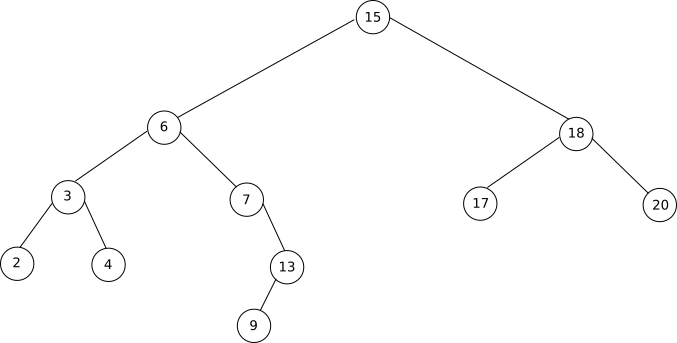
\includegraphics[width=0.8\textwidth]{./Images/arbre} %rajouter image du menu
	\caption{Exemple de la configuration possible d'une partie}
\end{figure}\vspace{0.2cm}

\subsection{Les règles et le déroulement d'une partie de Dames}

Chaque pièce doit se déplacer diagonalement. Un pion se déplace obligatoirement vers l’avant, en diagonale, d’une case sur une case libre de la rangée suivante. Lorsqu'il atteint la dernière rangée, le pion devient Dame. Une Dames doit attendre que l’adversaire ait joué au moins une fois avant d’entrer en action. Une Dame peut se déplacer en arrière ou en avant sur les cases libres successives de la diagonale qu’elle occupe. Elle peut donc se poser, tant que les cases précédentes sont vides, sur une case libre éloignée.\\

Lorsqu’un pion se trouve en présence, diagonalement, d’une pièce adverse derrière laquelle se trouve une case libre, il peut sauter par-dessus cette pièce et occuper la case libre. La pièce adverse est alors enlevée du damier. Cette opération complète est la prise par un pion. Lorsqu’une Dame se trouve en présence sur la même diagonale, directement ou à distance, d’une pièce adverse derrière laquelle se trouvent une ou plusieurs cases libres, elle peut passer par-dessus cette pièce et occuper, au choix, une des cases libres. Cette pièce est alors enlevée du damier. Cette opération complète est la prise par une Dame.\\

Lorsqu’au cours d’une prise par un pion, celui-ci se trouve à nouveau en présence, diagonalement, d’une pièce adverse derrière laquelle se trouve une case libre, il doit obligatoirement sauter par-dessus cette seconde pièce, voire d’une troisième et ainsi de suite, et occuper la case libre se trouvant derrière la dernière pièce capturée. 
Les pièces adverses ainsi capturées sont ensuite enlevées du damier dans l’ordre de la prise. Cette opération complète est une rafle par un pion.

Pour augmenter les différentes parties possibles et faire travailler notre IA dans des cas différents, nous avons laissé la possibilité que la prise soit obligatoire. 

 Lorsqu’au cours d’une prise par une Dame, celle-ci se trouve à nouveau en présence, sur une même diagonale, d’une pièce adverse derrière laquelle se trouve une ou plusieurs cases libres, elle doit obligatoirement sauter par-dessus cette seconde pièce, voire d’une troisième et ainsi de suite, et occuper au choix une case libre se trouvant derrière et sur la même diagonale que la dernière pièce capturée. Les pièces adverses ainsi capturées sont ensuite enlevées du damier dans l’ordre de la prise. Cette opération complète est une rafle par une Dame. Au cours d’une rafle, il est interdit de passer au-dessus d'une ou plusieurs de ses propres pièces. Au cours d’une rafle, il est permis de passer plusieurs fois sur une même case libre mais il est interdit de passer plus d’une fois au-dessus d’une même pièce adverse.\\

\begin{figure}[H]
	\center
	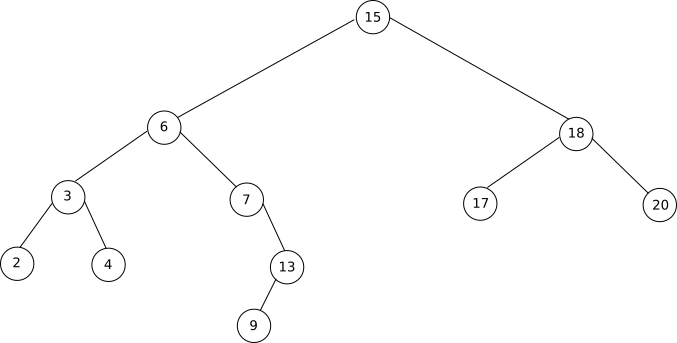
\includegraphics[width=0.8\textwidth]{./Images/arbre} %rajouter image Chloé
	\caption{Exemple de rafle par une dame}
\end{figure}\vspace{0.2cm}

Le jeu se termine lorsqu'un des joueurs ne possèdent plus de pièce ou ne peut plus en bouger aucune. L'adversaire remporte alors la partie.

\section{Implémentation du jeu}

 Nous allons ensuite vous présenter les classes qui constituent l'implémentation du jeu (hors IA et AlgoMinMax présenté dans la prochaine partie )

\subsection{Case}

La classe \textit{Case} représente tout simplement une case du plateau du jeu de Dames. Elle possède comme attributs des coordonnées, une couleur, une pièce qui peut être vide et plusieurs booléens qui ont un rôle dans l'implémentation et la partie graphique du jeu.
  
\subsection{Coordonnées}

La classe \textit{Coordonnées} possède deux entiers x,y représentant juste des coordonnées sur le plateau. Nous avons créé cette classe pour ne pas avoir à transporter deux variables à chaque fois.

\subsection{Couleur}

Cette classe sert à différencier la couleur d'une pièce, d'un tableau de pièce, d'un joueur ou d'une case.

\subsection{Damier}

La classe \textit{Damier} est la classe graphique du jeu de Dames. Elle représente le plateau du jeu. Il contient les tableaux de pièces du jeu, celui des cases du jeu, la taille du plateau ainsi que plusieurs booléens jouant un rôle dans les règles du jeu et son déroulement. %la procédure d'affichage elle n'y est plus ?

\subsection{Joueur}

La classe \textit{Joueur} représente un des deux joueurs du jeu. Elle se décline en deux classes qui héritent de joueur : \textit{IA} et \textit{Humain}. La classe \textit{Humain} n'a pas de différence avec la classe IA si ce n'est qu'il peut choisir son pseudo. En revanche la classe \textit{IA} contient d'avantages de méthodes, notamment la méthode \textit{Min-Max} et \textit{tourOrdi} qui seront expliquées ultérieurement. On retrouve également la procédure \textit{AJoue} qui simule le coup d'un joueur dans le jeu, ainsi que \textit{APerdu} qui retourne vrai ou faux selon si le joueur a perdu ou gagné la partie.

\subsection{Lanceur}

Cette classe constitue le \textit{Main} de notre programme, il est possible d'y modifier certains paramètre de la partie manuellement (si le menu n'est activé), sinon nous utilisons une autre classe que nous allons voir pour laisser le joueur décider des règles du jeu, celle-ci dessous, la classe Menu.

\subsection{Menu}

La classe \textit{Menu} permet de laisser l'utilisateur choisir ses règles pour la partie. Elle consiste simplement en un menu à choix multiples que l'on récupère et que l'on transmet au \textit{main} pour lancer la partie (exemple plus haut dans la partie sur les règles).

\subsection{Piece}

La classe \textit{Piece} correspond à une pièce du jeu. Elle se décompose en deux classes qui héritent de celle-ci : Pion et Reine (Une dame), qui sont les deux types différents de pièces qu'on retrouve dans le jeu de Dames. Dans cette version de notre jeu, c'est au niveau de la pièce que l'on vérifie si elle peut être mangée ou non, si elle peut manger une autre pièce ou non ainsi qu'afficher les déplacements possibles de la pièce sur le damier qu'elle contient directement.

\subsection{TableauPiece}

La classe \textit{TableauPiece} gère la liste des pièces d'un joueur, d'un camp comme de l'autre.

\subsection{Souris}

La classe \textit{Souris} sert à récupérer les actions de la souris pour permettre au joueur d'utiliser une souris pour jouer au lieu du clavier. Elle permet essentiellement de récupérer les coordonnées de la case sur laquelle le joueur clique. 


\section{Implémentation de la partie IA}

Nous allons maintenant nous intéresser davantage à la partie IA du projet. Il s'agit de la partie la plus importante car c'est sur elle que se porte le projet.  Nous allons détailler les classes du programme qui jouent un rôle dans l'IA basée sur l'algorithme Min-Max ainsi que certaines procédures importantes.
Dans un soucis de portabilité et de séparations des parties, nous avons séparé au maximum les deux parties, l'IA et l'algoMinMax pouvant être appliqué à d'autres jeux. Ce n'est ici pas tout à fait le cas mais c'est une piste d'amélioration.
 L'algorithme est appliqué à un arbre de nœuds, expliquons alors ce qu'est un nœud dans notre cas de figure, puis expliquons la création de l'arbre petit à petit .

\subsection{NoeudDame}

La classe \textit{NoeudDame} représente un "nœud" dans le cadre de l'algorithme Min-Max. Elle hérite de la classe abstraite \textit{Nœud} qui contient seulement la signature de la méthode \textit{Heuristique} que l'on détaillera dans la suite. 


Nous avons défini la "valeur" du nœud comme un \textit{Damier} du jeu de Dames. Ainsi, on pourra lui attribuer un certain "poids" grâce à la méthode \textit{Heuristique}.\\ 
L'intérêt est ensuite de pouvoir travailler avec ces poids (leur heuristiques) et choisir le meilleur coup possible.

Un objet \textit{NoeudDame} possède une liste de \textit{NoeudDame} correspondant aux successeurs du nœud, on les appellera également ses fils. La classe possède un entier profondeur permettant de savoir à quelle profondeur le nœud se situe dans l'arbre, la profondeur zéro étant celle de la racine. Nous avons travaillé sur les arbres en utilisant les schémas vu en cours pour la structure lorsque c'était possible.
Outre la fonction Heuristique que nous présentons ci-dessous et que nous détaillerons dans la partie discussion sur les Heuristiques, cette classe comprend les getters et setters.

Détaillons maintenant une des méthodes les plus importantes pour notre IA appartenant à cette classe : la méthode \textit{Heuristique}.
Son fonctionnement sera détaillé dans la partie discussion sur les Heuristiques

\subsubsection{L'heuristique}

%\begin{algorithm}
%	\caption{Heuristique(E :Couleur couleurordi) : Entier}
%	\begin{algorithmic}
%		\State  Entier res $\leftarrow$ 0;
%			\State booleen ordiBlanc $\leftarrow$ false;
%		\If (couleurOrdi est Couleur.Blanc) 
%		\State ordiBlanc $\leftarrow$ vrai;
		%\EndIf
	%	\If{noeud est une feuille}
	%	\State retourner l'heuristique du nœud
	%	\EndIf
	%	\If{profondeur du fils est paire}
	%	\State valeur $\leftarrow$ -$\infty$
	%	\For{chaque fils de noeud}
	%	\State temporaire $\leftarrow$ minMax(fils,ProfondeurArbre,)
	%	\If{temporaire>valeur}
	%	\State valeur $\leftarrow$ temporaire
	%	\EndIf
	%	\EndFor
%		\Else
	%	\State valeur $\leftarrow$ $\infty$
	%	\State temporaire $\leftarrow$ minMax(fils,ProfondeurArbre,)
	%	\If{temporaire<valeur}
	%%	\State valeur $\leftarrow$ temporaire
	%	\EndIf
	%	\EndIf
%	\end{algorithmic}
%\end{algorithm}\vspace{0.4cm}



\subsection{Arbre}

\begin{figure}[H]
	\center
	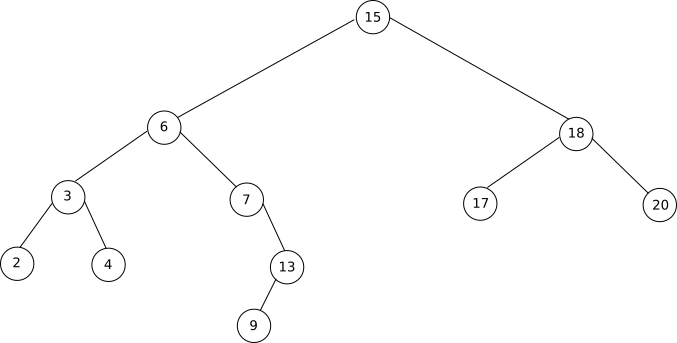
\includegraphics[width=0.8\textwidth]{./Images/arbre}
	\caption{Exemple d'un arbre quelconque}
\end{figure}\vspace{0.2cm}


La classe \textit{Arbre} représente l'arbre sur lequel se base notre algorithme Min-Max. Dans l'exemple du dessus cet arbre est binaire, le notre ne l'est absolument pas puisque chaque branche représente un damier possible que le joueur peut créer en jouant une de ses pièces. Chaque rond représente un nœud et la valeur à l'intérieur correspond à la valeur du nœud. Cette valeur est le "poids" du damier appartenant au nœud, c'est le résultat de la méthode \textit{Heuristique}.\\

La classe contient en attribut un nœud qui est en faite le nœud racine de l'arbre. Il est de profondeur 0. On accède au reste de l'arbre grâce à la liste de successeurs que le nœud racine possède. La classe comprend également \uline{la profondeur de l'arbre correspondant en pratique au nombre de coup à l'avance que l'IA peut anticiper}. Nous allons maintenant détailler la création de l'arbre grâce aux trois méthodes suivantes.\\

\subsubsection{ListeDesCoupsPossibles : Coordonnees[]}

Cette méthode permet de retourner un tableau de \textit{Coordonnees}. Chaque coordonnée du tableau correspond à un déplacement possible de la pièce mis en paramètre de la méthode. Ainsi, la méthode retourne l'ensemble des "coups" possibles à partir d'une pièce.

\subsubsection{GenererArbreParPiece : void}

Cette méthode permet à partir d'un nœud\_0 de créer un fils nœud\_1 puis de l'ajouter à la liste des successeurs du nœud\_0. Elle va en réalité évaluer le déplacement de la pièce grâce à la méthode \textit{ListeDesCoupsPossibles}. Pour chaque valeur du tableau de coordonnées elle va générer un nœud de profondeur +1 avec le damier comprenant le déplacement de la pièce. Si la pièce vient de manger une pièce adverse et peut en manger au moins une autre, alors cette même méthode est appelé sur ce nœud qui vient d'être créé et ainsi de suite (récursivité). Une fois que la pièce ne peut plus manger, si le nœud est une feuille de l'arbre alors ce nœud est ajouté à la liste des successeurs du nœud entré en paramètre de la méthode \textit{GenererArbreParPiece}, sinon on appelle la méthode \textit{GenererArbreParNoeud} (détaillée juste après) sur ce nœud généré pour enfin l'ajouter au nœud entré en paramètre de la méthode \textit{GenererArbreParPiece}. 

\subsubsection{GenererArbreParNoeud : void}

Cette méthode est la méthode principale de la création de l'arbre. Elle est appelée sur chaque nœud dont nous voulons connaître leur fils. Elle est notamment appelée sur l'attribut \textit{racine} de la classe \textit{Arbre} qui est un \textit{NoeudDame}. La méthode va en réalité, selon la profondeur du nœud, appeler pour chaque pièce du tableau de pièce du damier la méthode \textit{GenererArbreParPiece}. Elle permet simplement de découper le problème "en petits morceaux" pièce par pièce. C'est uniquement la méthode \textit{GenererArbreParPiece} qui va ajouter des successeurs au nœud. Les deux méthodes s'appellent mutuellement jusqu'à ce que le nœud soit une feuille de l'arbre.

\subsection{Coup}

La classe \textit{Coup} représente un coup pour une pièce du jeu. Elle  contient deux pièces : celle au départ (avant déplacement) du coup et celle à la fin (après le coup). Évidemment ce qui va changer entre les deux pièces sont les coordonnées de la pièce et le statut (un pion peut devenir une reine).

\subsection{Resultat\_minMax}

Cette classe a été créée pour exploiter le résultat retourné par notre méthode min-max. Elle n'a pas de signification particulière et est juste une manière pratique de transporter les données. Pour résumer, elle comprend la valeur d'un nœud et également la liste de coups associée à cette valeur. C'est une classe pratique pour notre implémentation.

\subsection{IA}

La classe \textit{IA} hérite de la classe \textit{Joueur} et représente un ordinateur doté d'une intelligence artificielle. C'est dans cette classe que l'on retrouve l'algorithme Min-Max que nous allons détailler ci-dessous. Tout d'abord nous allons écrire en pseudo-code la méthode \textit{minMax}, puis nous allons expliciter son fonctionnement. Nous verrons ensuite la méthode \textit{tourOrdiIA}, son pseudo-code et son explication.

\subsubsection{minMax : Resultat\_minMax}

%\begin{algorithm}
%	\caption{minMax(E : NoeudDame noeud; entier profondeurArbre) : Resultat\_minMax}
%	\begin{algorithmic}
%	\If{noeud est une feuille}
%		\State retourner l'heuristique du nœud
%	\EndIf
%	\If{profondeur du fils est paire}
%		\State valeur $\leftarrow$ -$\infty$
%%		\For{chaque fils de noeud}
%			\State temporaire $\leftarrow$ minMax(fils,ProfondeurArbre,)
%			\If{temporaire>valeur}
%				\State valeur $\leftarrow$ temporaire
%			\EndIf
%		\EndFor
%	\Else
%		\State valeur $\leftarrow$ $\infty$
%		\State temporaire $\leftarrow$ minMax(fils,ProfondeurArbre,)
%		\If{temporaire<valeur}
%			\State valeur $\leftarrow$ temporaire
%		\EndIf
%	\EndIf
%	\end{algorithmic}
%
%\vspace{0.4cm}


L'algorithme minMax à partir d'un arbre dont les nœuds sont des damiers du jeu de Dames doit ressortir le meilleur coup à jouer pour l'ordinateur.\\

On part de la racine qui représente le damier actuel, chacun des nœuds fils d'un nœud représente une situation possible avec un coup d'écart avec le nœud père. La profondeur de l'arbre qu'on explore va avoir un lien direct avec la difficulté de l'ordinateur. Plus l'arbre est profond plus l'ordinateur fera son choix en fonction des conséquences à plus long termes. Autrement dit la profondeur de l'arbre correspond au nombre de coup d'avance avec lequel joue l'ordinateur. \\

L'algorithme consiste à évaluer les feuilles de l'arbre grâce à la méthode \textit{Heuristique} en leur donnant une valeur représentative de l'intérêt de la situation pour le joueur. Ensuite en fonction de si le niveau auquel on se situe est paire ou impaire on remonte la valeur maximal ou minimal des fils au nœud père. A la fin on obtient le coup qui maximise l'intérêt pour l'ordinateur tout en minimisant l’intérêt pour l'adversaire. Plus la profondeur de l'arbre va être grande plus on va pouvoir voir cela à long terme.\\

L’algorithme semble parfait et imbattable si on pousse la profondeur au maximum, cependant le coût de calcul et la consommation de mémoire est exponentielle et on arrive rapidement aux limites de l'ordinateur même pour un jeu de Dames. Il existe donc certaines méthodes pour réduire le coût de calcul comme l'élagage alpha-bêta que nous n'avons pas eu le temps de mettre en place.\\

L'autre faille importante est que la méthode \textit{Heuristique} ne peut être parfaite et résulte entièrement de l'interprétation humaine. Intéressons nous maintenant à la méthode \textit{tourOrdiIA}.\\




%Le coeur de ce projet ce trouve dans cette partie. Nous avons d'abord
%fait un travail de recherches pour maîtriser ces concepts pour avancer
%ensuite plus rapidement et sereinement. Nous avons découpé notre travail
%comme présenté dans la partie 5 avec la modélisation UML.
%
%La fonction euristique est la pierre angulaire de cette partie, nous
%avons donc réfléchis et nous sommes renseignés sur les différentes
%positions (positions imprenables sur les côtés du plateau car les
%pions ne peuvent y être mangé ...) pour établir un ordre de priorité
%entre toutes et une valeur choisie sur une échelle de -5 pour la moins
%intéressante (position pour une Dames de se faire manger) et 14 pour
%la plus intéressante (faire une Dames). Cette échelle est encore sucesptible
%d'évoluer selon l'euristique que nous auront choisi puis si nous en
%testons plusieurs. Un seul déplacement peut en combiner plusieurs
%car un pion peut se mettre en position de manger et d'être manger
%aussi.
%
%L'action de manger étant obligatoire nous ne passont pas par la fonction
%euristique lorsque cette action se présente. C'est une des optimisations
%que nous comptons mettre en place.
%
%Nous avons aussi une fonction listecoups qui établit pour une composition
%donnée, une liste dynamique des positions possibles pour chaque pions.
%Cette liste est ensuite utilisée pour construire l'arbre vide sous
%forme de liste chainée puis de le remplir avec les valeurs des noeuds
%grâce à la fonction euristique.
%
%Enfin, nous avons la fonction parcoursminimax qui parcourt l'arbre
%avec l'algorithme minimax pour ressortir la branche la plus intéressante
%au niveau du gain.
%
%En bonus nous essayerons de rajouter la fonction élagage qui réalisera
%l'élagage détaillé dans les parties 3 et 4 juste avant la fonction
%parcoursminimax

\subsubsection{tourOrdiIA : void}

La méthode \textit{tourOrdiIA} représente le déroulement du tour de l'IA, concrètement ce que fait l'IA lorsque c'est à elle de jouer. On mettra ci-dessous le pseudo-code de la méthode puis nous allons expliquer en quoi elle consiste :

%\begin{algorithm}
%	\caption{tourOrdiIA(E : int difficulte; boolean tourBlanc) : void}
%	\begin{algorithmic}
%	\State \underline{Variables} : Arbre arbre, ArrayList<Coup> meilleurCoup, Entier indice,x,y
%	\State
%	\State arbre $\leftarrow$ Arbre(difficulte,this.couleur,this.damier,this.peutMangerEnArriere,this.obligerLesSauts)
%	\State meilleurCoup $\leftarrow$ minMax(arbre,tourBlanc,this.peutMangerEnArriere,this.obligerLesSauts).getListeDeCoup()
%	\State indice $\leftarrow$ 0
%	\State x $\leftarrow$ meilleurCoup.get(0).getPieceAvantD().getC().X()
%	\State y $\leftarrow$ meilleurCoup.get(0).getPieceAvantD().getC().Y()
%	\State this.Ajoue(x,y,tourBlanc,this.peutMangerEnArriere, this.obligerLesSauts)
%	\While{indice < taille du tableau meilleurCoup}
%	\State x $\leftarrow$ meilleurCoup.get(indice).getPieceApreD().getC().X()
%	\State y $\leftarrow$ meilleurCoup.get(indice).getPieceApresD().getC().Y()
%	\State this.Ajoue(x,y,tourBlanc,this.peutMangerEnArriere,this.obligerLesSauts);
%	\State indice $\leftarrow$ indice+1;
%	\EndWhile
%	\end{algorithmic}
%\end{algorithm}\vspace{0.4cm}

Dans un premier temps l'arbre est généré avec une profondeur \textit{difficulte}. C'est ainsi qu'on règle la difficulté de l'IA, il s'agit en effet de la profondeur de l'arbre. Concrètement, \uline{la difficulté de l'IA se résume au nombre de coups d'avance qu'elle a sur le damier actuel}. Ensuite le \textit{meilleurCoup} est récupéré grâce à la méthode \textit{minMax} où l'on va appeler l'accesseur \textit{getListeDeCoup} pour ainsi récupérer le tableau dynamique du ou des meilleur.s coup.s à jouer. On va alors "simuler" un clique sur la pièce initiale en récupérant ses coordonnées puis cliquer sur la liste des coups à jouer en utilisant le tableau de coups \textit{meilleurCoup}. Ce dernier est de dimension 1 lorsqu'il y a un déplacement sans prise de pièce, il sera de dimension supérieure s'il est dans une situation de saut multiple.

\section{Application de la méthode à des exemples}

Pour mieux comprendre cette méthode et les différents cas possibles,
voici plusieurs exemples (simplifier car on a choisit de représenter
deux pions sur plusieurs coups en ayant attribué des valeurs aux noeuds).

Pour simplifier l'exemple nous l'avons réalisé en trois parties:  d'abord l'explication de la méthode pour un pion et un de ses coups possibles et ensuite nous avons détaillé les possibilités sur plusieurs coups pour un plateau de jeu plus petit que le classique pour ne pas avoir un nombre de possibilité trop important, enfin nous avons détaillé le cas pour une dame avec une profondeur de deux pour montrer cette difficulté. 


\subsection{la méthode pour un pion sur un coup en utilisant notre Heuristique finale}
Dans ce cas nous allons traiter uniquement la méthode pour le pion blanc situé en (6,5) et sur une profondeur de 1. Le but est donc d'établir les nouvelles positions de ce pion en un seul coup. Pour chaque pion qui n'est pas une dame, ce nombre est d'au maximum deux si aucun pion ne peut-être mangé, 4 si il peut manger en arrière de chaque côté, que la situation se présente. 
Nous allons regarder ce cas: 

\begin{figure}[H]
	\center
	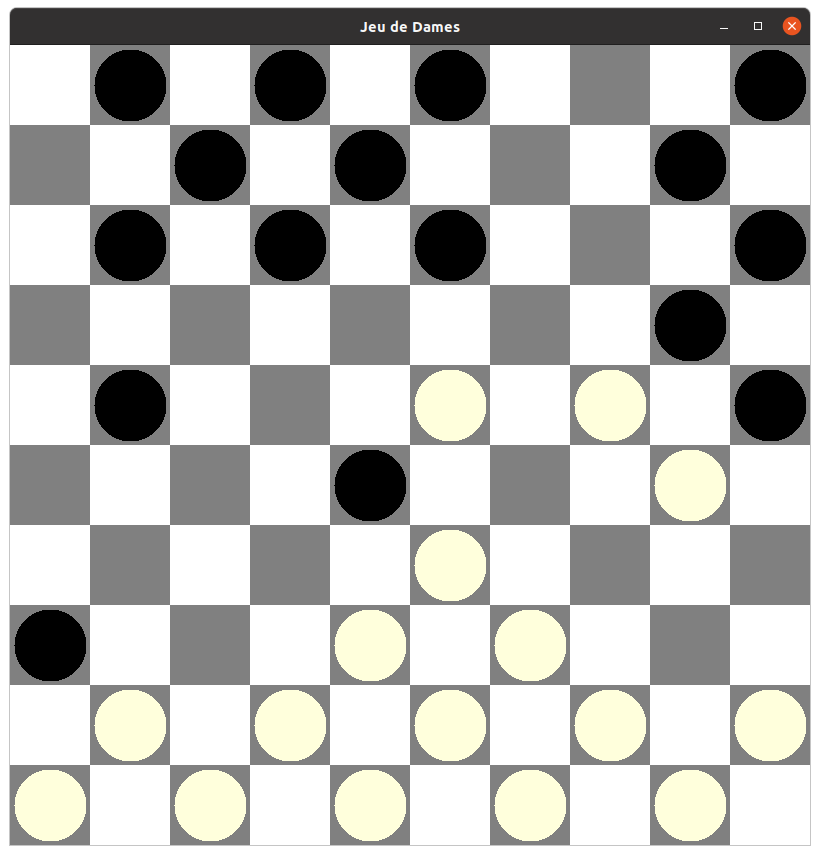
\includegraphics[width=0.8\textwidth]{./Images/image1heuristique} 
	\caption{Exemple de la configuration possible d'une partie}
\end{figure}\vspace{0.2cm}

Dans notre cas, le pion peut se déplacer en:
- (5,4) en avançant à gauche
- (7,4) en avançant à droite
- (4,7) en mangeant le pion en (5,6)


En calculant L'Heuristique de ce pion pour chacun de ses déplacements on obtient les correspondances suivantes.
- (5,4) et (7,4) obtiennent le même score car il y a toujours le même nom de pions pour les deux adversaires et de positions imprenables : -2
- (4,7) obtient meilleur score: car il y a un pion de moins pour l'adversaire, celui qui a été mangé, et autant de pion pour lui et de position imprenable pour les deux: 3.




On peut finalement en conclure qu'à la profondeur 1 le meilleur coup semple être (4,7). On obtient donc la situation suivante:

\begin{figure}[H]
	\center
	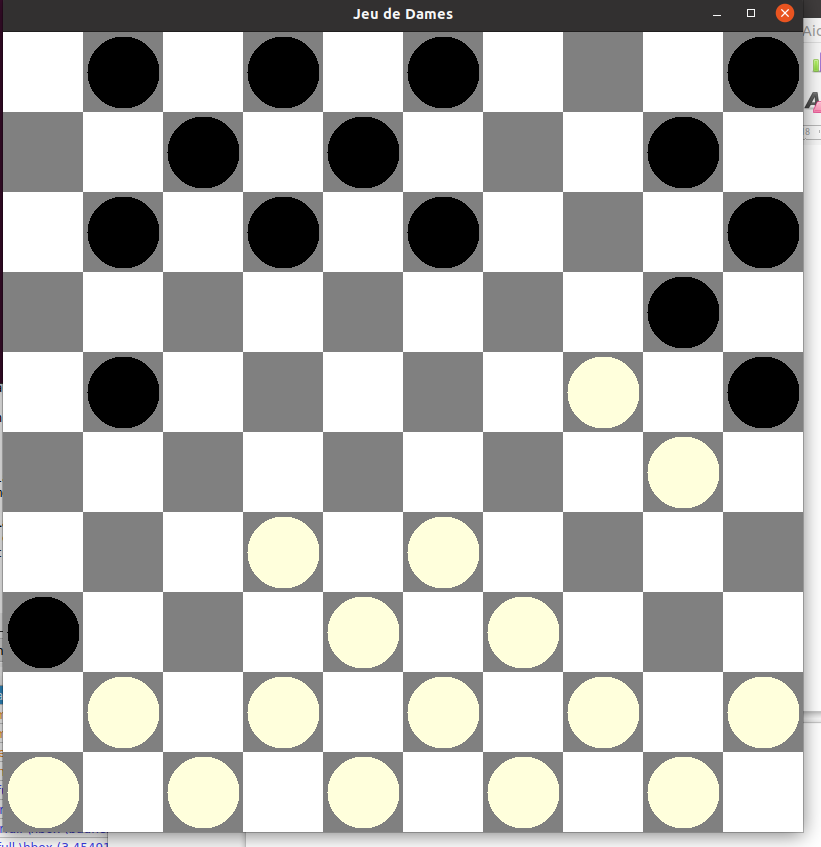
\includegraphics[width=0.8\textwidth]{./Images/image2heuristique} 
	\caption{Exemple de la configuration possible d'une partie}
\end{figure}\vspace{0.2cm}

Toutefois, le coup choisi lorsqu'on regarde à un coup n'est pas forcément le même que celui qui serait choisi à 5 coups, d'où l'intérêt de la profondeur.

\subsection{un exemple complet sur plateau 6x6}
Si on reprend une situation possible en étudiant tous les pions on peut se rendre compte que l'arbre se complexifie rapidement. 



\subsubsection{prodondeur 1} 
À la profondeur 1, le joueur en blanc peut choisir de jouer:
-(2,5) à (1,4)
-(2,5) à (3,4)
-(5,6) à (4,5)
-(6,5) à (5,4)


\subsubsection{prodondeur 2}
Pour étudier la profondeur 2, on ne va considérer que le coup 1 (2,5) à (1,4) a été réalisé, on travaille donc sur sa branche.
Les coups possibles pour l'adversaire en noir sont donc :
- (1,2) à (2,3)
- (4,1) à (3,2)

\subsubsection{prodondeur 3}
Enfin, selon le coup choisit par l'adversaire les coups possibles sont : 

si le coup - (1,2) à (2,3) est choisi; les possibles pour le joueur en blanc sont :
- (1,6) à (2,5)
- (5,6) à (4,5)
- (6,5) à (5,4)

Toutes ces positions ne changent pas le nombre de pions des deux joueurs et diminuent de 1 pour chacune le nombre de position imprenable. L'IA choisira donc un de ces choix par défaut.

\begin{figure}[H]
	\center
	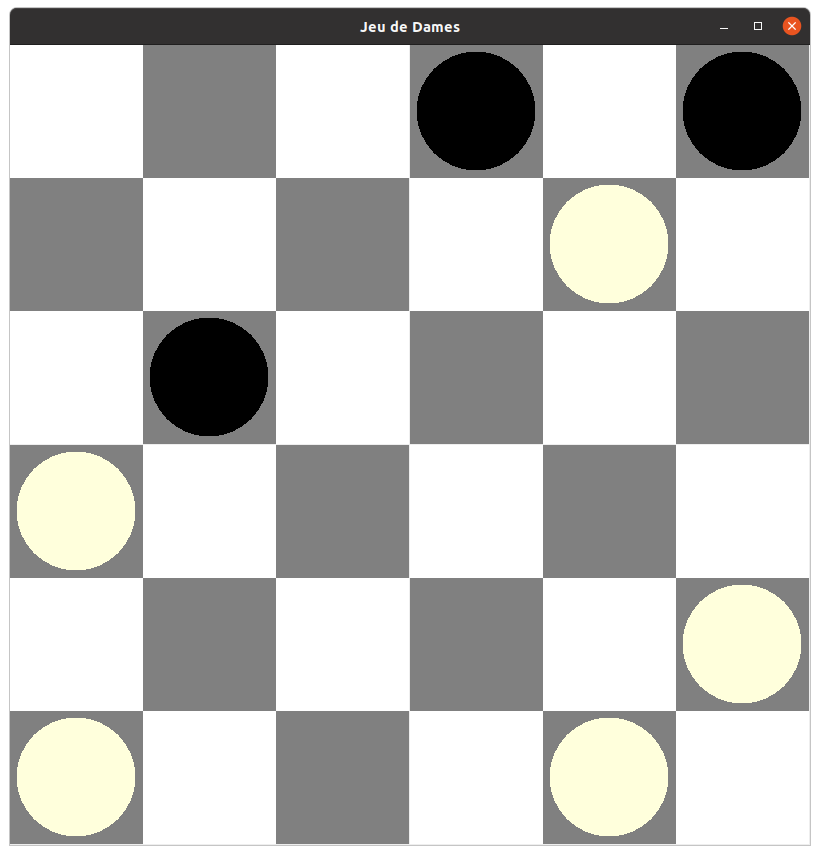
\includegraphics[width=0.8\textwidth]{./Images/image3heuristique} 
	\caption{Exemple de la configuration possible d'une partie}
\end{figure}\vspace{0.2cm}

Cet exemple montre l'intérêt d'aller voir à plusieurs coups à l'avance car si le pion en  (1,6) passe en (2,5) puis en (3,4) le joueur blanc perdra l'avantage car il sacrifiera ce pion au tour d'avant. Alors que si le pion en (6,5) se déplace tout le long de sa diagonale il pourra faire une dame.

\subsection{la méthode pour une dame}
Pour une dame, le nombre de coup possible est beaucoup plus important car elle peut se déplacer sur toutes les cases de ses diagonales vides et manger des pions si ceux ci sont sur ces diagonales et la case suivante est libre.

L'heuristique est appliquée sur chaque valeur. Il est donc logique que lorsqu'on regarde sur plusieurs coups l'arbre des possibilités gonfle de manière exponentielle. Il est d'ailleurs possible d'afficher les damiers possibles sur le nombre de coup à la demande, dans le lanceur.


\chapter{Discussion sur les Heuristiques}
\section{Notre idée d'origine}

Dès le début de notre projet, avant même de commencer à coder nous avons réfléchi à cette Heuristique. En effet, même si notre programme est très performant au niveau de la mémoire si l'Heuristique n'est pas précise ou n'est pas adaptée au jeu de Dames, notre IA n'arrivera pas à gagner.
Nous avons donc fait des recherches et surtout nous avons réfléchi  à toutes les possibilités que peut rencontrer un pion durant un jeu de Dames en y jouant plusieurs fois. Nous avons dressé une liste très complète des positions possibles et de leurs caractéristiques:

- manger un pion

- manger plusieurs pions

- être en position de manger au prochain coup un ou plusieurs pions

- être en position de se faire manger (en étant un pion ou une dame ça ne sera pas la même valeur)

- position de faire une dame (arriver sur la dernière ligne du camp de l'adversaire)

- manger une Dame

- position imprenable
 
 -position neutre (ne pas pouvoir être mangé et avoir simplement gagné du terrain)

Après avoir réaliser cette liste (qui n'est bien sûr pas exhaustive), la difficulté suivante a été de quantifié et donc déjà de classer ces différentes positions:
Nous avons opté pour ce choix:
dans les positions à privilégier:
- manger une Dame

- faire une Dame

- manger plusieurs pions

- position de manger au prochain tour

-position imprenable

-position neutre

- position de se faire manger une Dame

-position de se faire manger au prochain tour (être en danger)


Ensuite, il faudrait réfléchir à une échelle pour savoir quelle Heuristique choisir pour quelle position, en effet, combien vaut "manger une Dame" par rapport à manger un ou plusieurs pions, 3 fois plus ? 2 fois plus ?
Nous avons donc implémenter cette proposition en faisant varier les valeurs d'Heuristique pour trouver une qui pourrait nous convaincre déjà à l'ordre 1 (un coup à l'avance ).


\subsection{une proposition à la profondeur 1}

%\begin{algorithm}
%	\caption{tourOrdiIA(E : int difficulte; boolean tourBlanc) : void}
%	\begin{algorithmic}
%	\State \underline{Variables} : Arbre arbre, ArrayList<Coup> meilleurCoup, Entier indice,x,y
%	\State
%	\State 
%	\end{algorithmic}
%\end{algorithm}\vspace{0.4cm}

\subsection{L'Heuristique finale}
Nous avons énormément fait travaillé l'Heuristique précédente et nous nous sommes rendues compte que tous ces tests étaient très coûteux et prenaient du temps.
Nous avons essayé d'en faire moins et nous avons repris toute notre liste de position possible, nous avons gardé position imprenable. Position neutre n'était pas forcément utile et on aurait pu lui affecter la valeur 0 car elle ne fait pas réellement avancer le jeu, en effet, un pion qui avance, seul devient souvent au bout de plusieurs coups un pion en danger. Nous l'avons donc enlever. 
La position de se faire manger au prochaine tour (c'est à dire que le pion est en danger) correspond lorsque l'on voit à plusieurs coups à comparer le nombre de pions présent au tour d'après. En effectuant un compte de pions sur plus d'un coup, bien plus simple à tester, on se retrouve avec le même résultat. Pareil pour le fait d'être en position de manger un pion de l'adversaire, si au tour d'après l'adversaire a un pion de moins, c'est qu'on a pu le manger.
En mettant en place un compte du nombre de pions présent sur l'échiquier, on a pu enlever position de se faire manger, position de manger et l'action de manger. Il en est de même avec les Reines en mettant en place un compte séparé pour les Reines et les pions en mutilipliant le nombre de Reines par 20 et le nombre de Pions par 5. 
Il nous reste donc la position imprenable et les deux compteurs de Pions et de Reines. En ajoutant ces valeurs, on obtient l'Heuristique recherchée. Une Heuristique plus simple nous a permis de réaliser l'algorithme Min-Max sur d'avantage de coups (jusqu'à 5 au maximum) quasiment en instantané.


%% rajouter Heuristique finale en pseudo code

\chapter{UML}

\section{diagramme de cas d'utilisation}

\begin{figure}[H]
	\center
	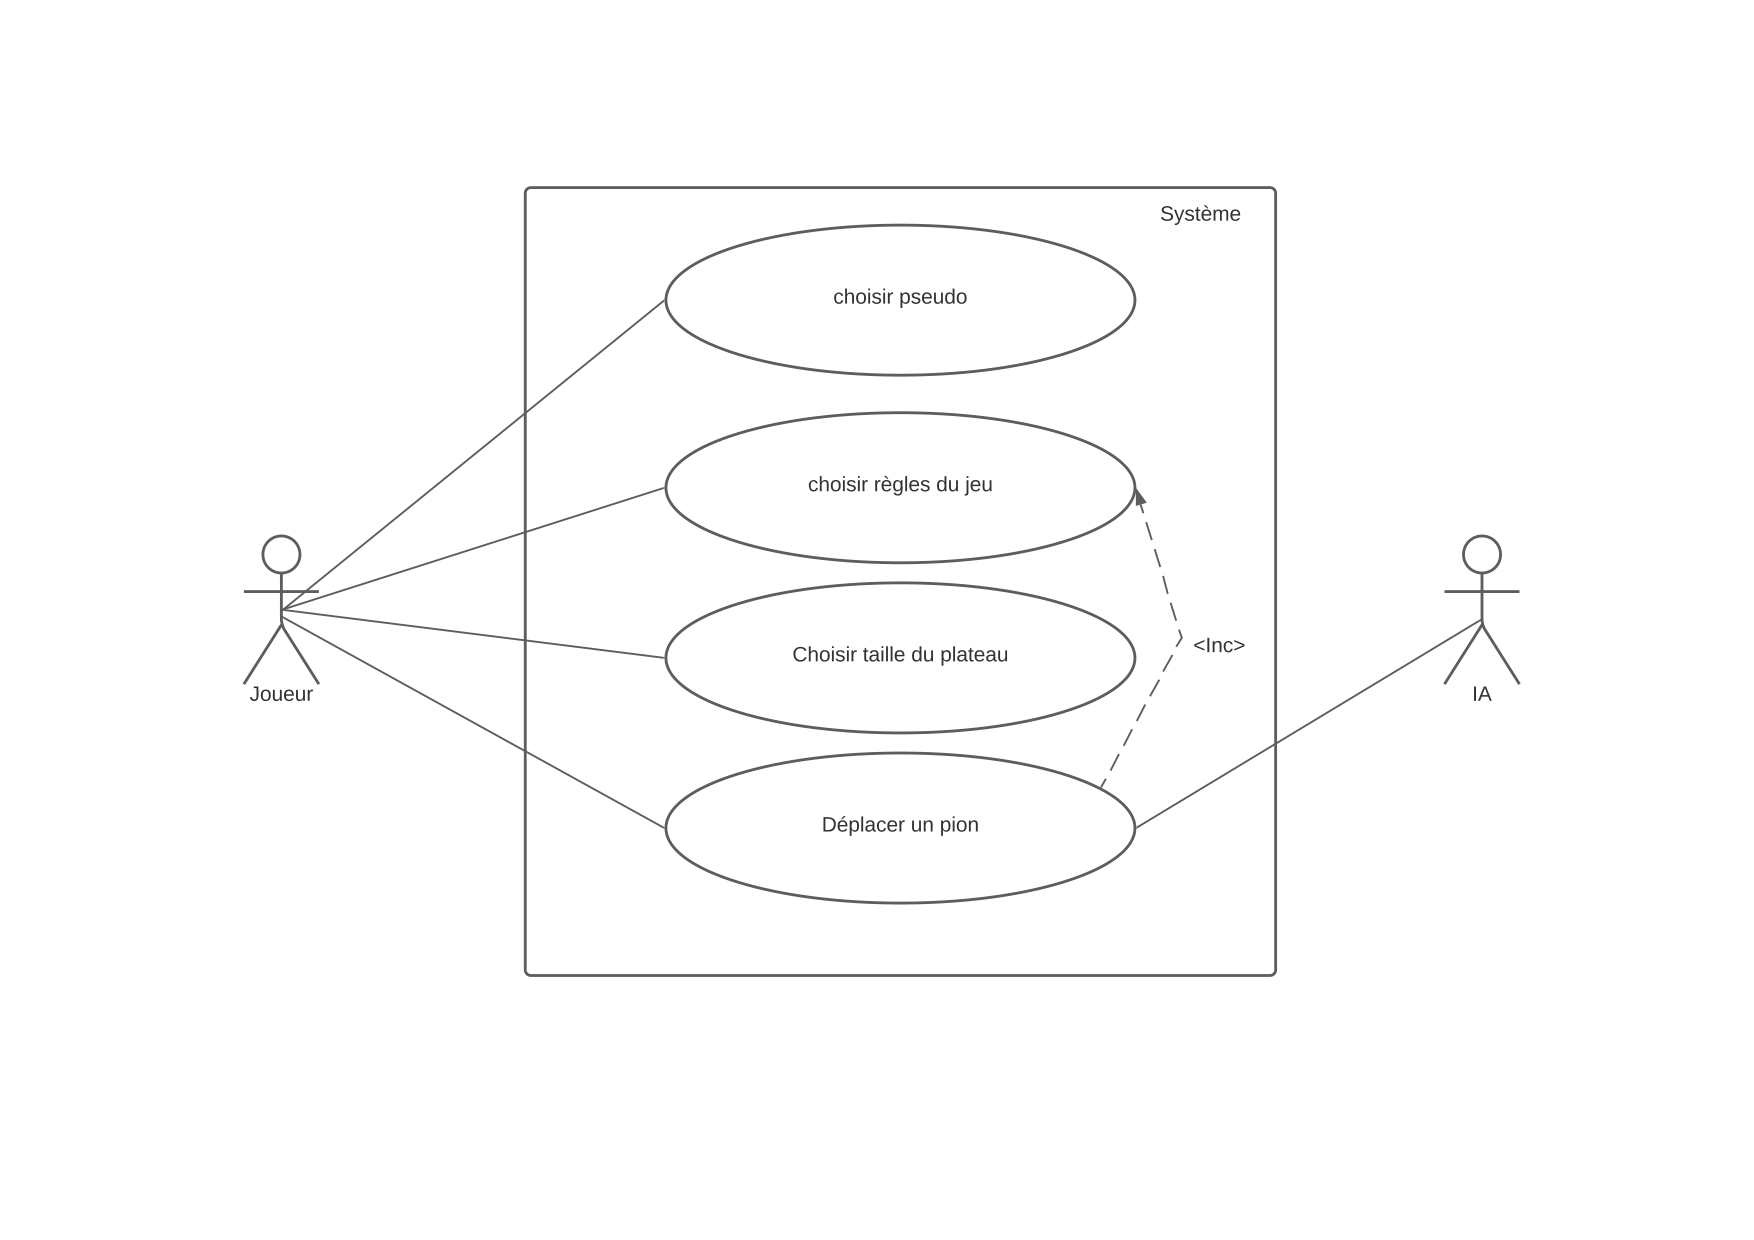
\includegraphics[width=1\textwidth]{./Images/Diagramme_use_case}
	\caption{Diagramme use case du jeu de Dames}
\end{figure}\vspace{0.2cm}

L'utilisateur

\section{diagramme de séquences}

Nous avons réalisé plusieurs diagrammes de séquences pour détailler
la partie algorithme Min-max, selon les différentes situations possibles:

\begin{figure}[H]
	\center
	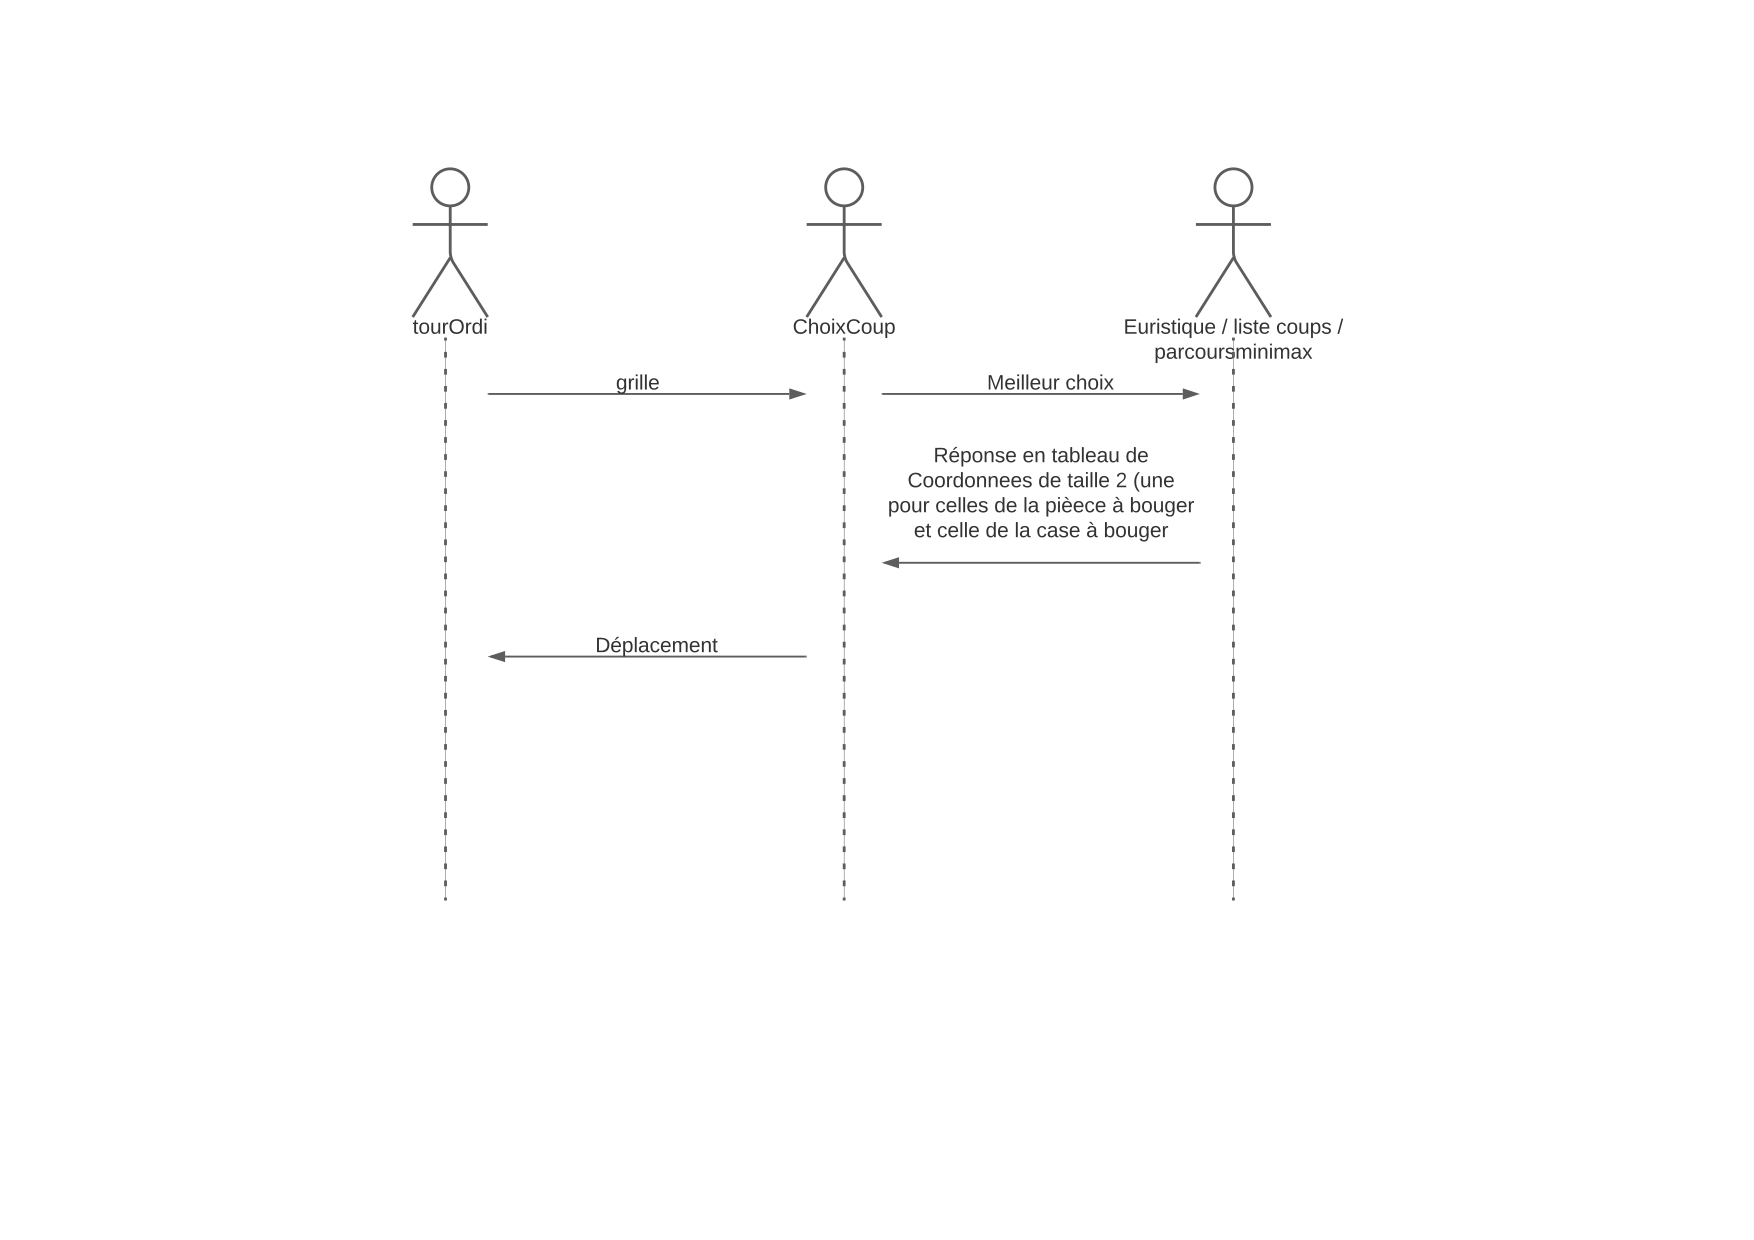
\includegraphics[width=0.8\textwidth]{./Images/Diagramme_de_sequence1}
	\caption{Diagramme de séquence choix coup ordi}
\end{figure}\vspace{0.2cm}

\begin{figure}[H]
	\center
	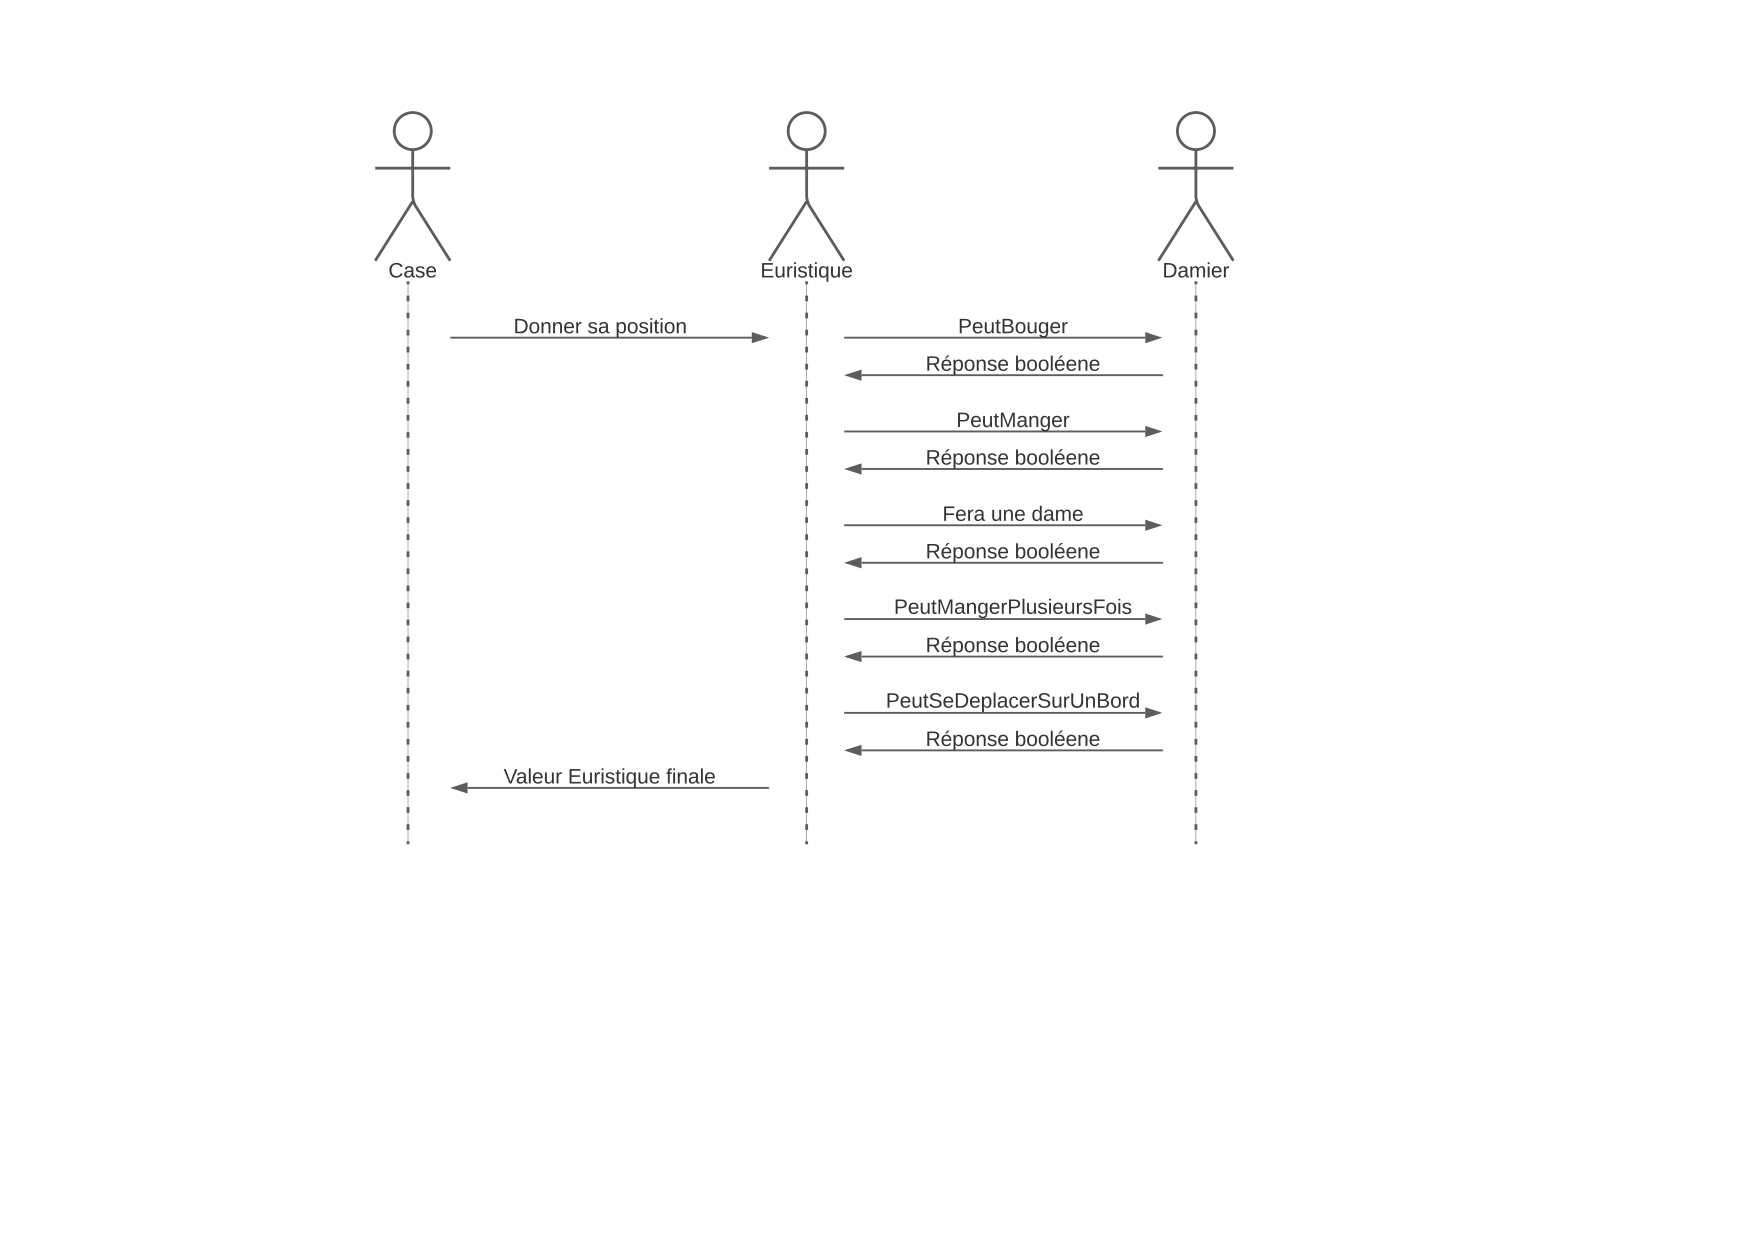
\includegraphics[width=0.8\textwidth]{./Images/Diagramme_de_sequence2}
	\caption{Diagramme de séquence heuristique}
\end{figure}\vspace{0.2cm}

\section{diagramme de classes}

\begin{figure}[H]
	\center
	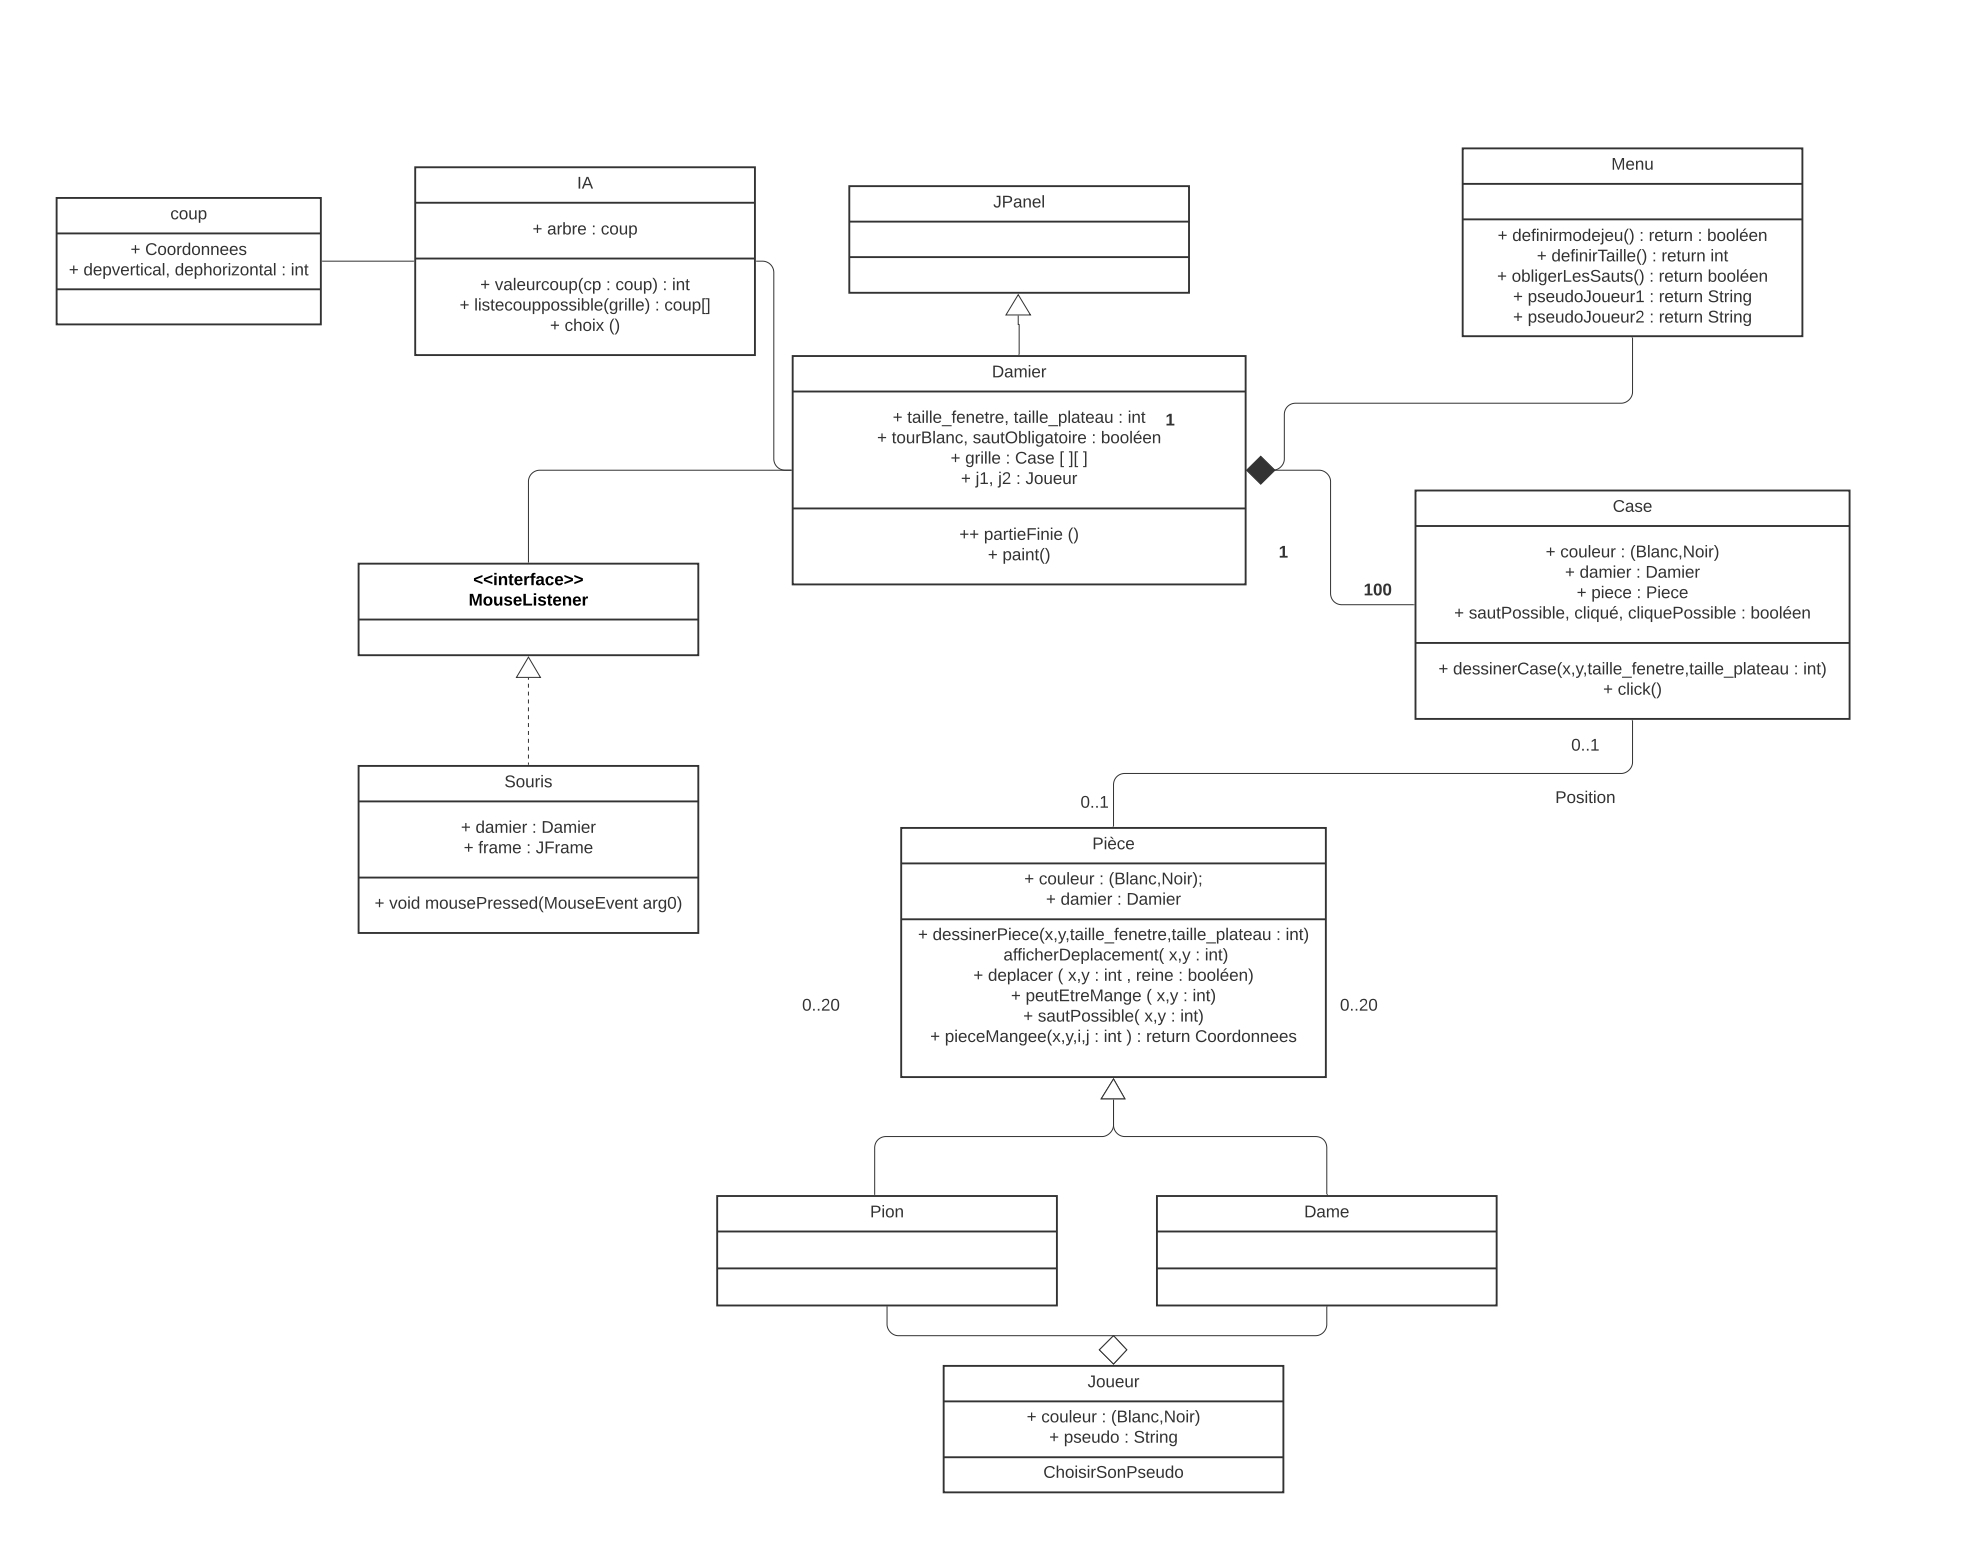
\includegraphics[width=1\textwidth]{./Images/Diagramme_classe}
	\caption{Diagramme des classes}
\end{figure}\vspace{0.2cm}

%\loadgame{\string"Diagramme UML\string"}\showboard

Notre diagramme de classe a beaucoup évolué tout au long de notre projet, il se sépare en deux parties, comme nous avons détaillé dans les deux parties implémentation plus haut.
Ce diagramme met aussi en évidence notre utilisation des interfaces pour rendre notre code plus portatif. Nous avons aussi essayé de découper notre programme en le structurant comme la Programmation Orientée Objet le demande. Les classes non triviales ont été détaillée plus haut.



\chapter{Problèmes rencontrés}

Le premier problème rencontré est lors de l'ajout d'un joueur IA. Notre programme n'était pas du tout destiné à jouer automatiquement. Le programme devait attendre un "clique" souris pour continuer à s'exécuter. Ne pouvant pas simuler un "clique souris" il nous a fallu revoir tout le corps du \textit{Main} ainsi que de nombreuses méthodes.\\

Le second est lors de la création de l'arbre. La manipulation d'objet étant en réalité une manipulation d'adresse, lorsque nous voulions travailler sur une copie du damier en affectant directement un damier à un autre, nous nous retrouvions à modifier le damier de base, alors que ce n'était pas le but. Grâce à l'utilisation d'une classe implémentée \textit{Cloneable}, cela nous a permis de "cloner" nos objets, de sorte à les copier et ne modifier que les copies de manière à laisser intact les originaux. Une fois cela compris la profondeur 1 a été plus ou moins facile à faire. En effet, lors des sauts multiples il a fallu faire appel à une récursivité de loin triviale. Les problèmes se compliquent pour générer un arbre de dimension $n$. En effet, la gestion de couleur des pièces change, et nous remarquons que nous devons appliquer une récursivité non pas seulement sur les pièces mais sur chaque nœud. Une réorganisation du code avec la création de méthodes fût nécessaire afin de permettre le bon déroulement de la méthode. Il a également fallu trouver un moyen d'afficher le damier des nœuds d'une certaine profondeur de manière à pouvoir observer et remarquer les éventuels oublis. La création de l'arbre reste de loin le problème le plus dur rencontré dans ce projet.\\

Le troisième problème rencontré est lors de la méthode \textit{minMax}. L'originale consiste à seulement renvoyer la valeur de la feuille de l'arbre qui maximise les coups du joueur tout en minimisant ceux des adversaires, alors que ce qui nous intéresse vraiment c'est le meilleur coup à partir du damier actuel. Il a fallu adapter un peu l'algorithme original pour ainsi renvoyer la valeur des nœuds et la meilleure liste de coups.\\

Enfin le dernier problème rencontrer est le choix de l'heuristique. Une infinité peut en être créée. Quelles situations privilégier ? Pourquoi une plus qu'une autre ?Nous en avons débattu naturellement, mais nous avons fini par en choisir une, à grand renfort de test de parties, souvent plusieurs dizaine de fois. Notre choix s'est porté sur celle qui nous semble la plus adaptée au jeu de Dames. Aujourd'hui en jouant contre une IA de niveau 5 nous n'arrivons plus à gagner.



\chapter*{Conclusion:}

Pour commencer ce projet a été très enrichissant pour nous tous d'un point de vue informatique et programmation. En effet il nous a permis d'implémenter et de se familiariser avec de nouvelles structures de données que nous avions étudiées en cours cette année. Notamment les structures du type arbre restaient assez floues dans notre esprit et ce projet nous a permis de nous familiariser avec cette notion qui nous sera forcément utile à l'avenir.\\
De plus ce projet nous a permis de découvrir ou d'approfondir nos connaissances sur la théorie des jeux à somme nulle et comment on pouvait implémenter une intelligence artificielle sur ce type de jeu. Car ce qui fonctionne pour le jeu de dame avec l'algorithme min-max est facilement transposable à n'importe quelle jeu de ce type tel qu'un morpion ou de façon plus complexe le jeu d'échec.\\

D'autre part nous étions assez familier avec le jeu de dame, premièrement car c'est un jeu auquel nous avions déjà tous joué et deuxièmement pour une partie du groupe nous avions auparavant travaillé sur un jeu de dame sans intelligence artificielle auquel nous pouvions joué manuellement. Cependant il s'est révélé comme toujours beaucoup plus complexe que nous le pensions d'y ajouter une intelligence artificielle et nous avons rencontré de nombreux problèmes mais nous en avons déjà parlé ci-dessus.\\

Nous avons souhaité conserver l'interface graphique de notre jeu afin de donner une expérience plus sympathique et plus visuel à l'utilisateur. Nous l'avions déjà développé pour l'ancien jeu mais il a fallu effectuer certaines modification pour y ajouter l'intelligence artificielle.\\

Enfin la principale différence que nous avons rencontré par rapport à l'an dernier est de se retrouver avec un groupe plus conséquent passant de deux à trois personnes. Nous avions tous pris l'habitude de travailler par groupe de deux l'an dernier mais l'ajout d'une troisième personne nous a obligé à être encore plus organisé et à l'écoute des uns des autres car nous avions encore plus d'idées et de points de vue différents qu'il fallait concilier. C'est le point fort et le point faible du travail de groupe mais finalement nous avons rapidement réussi à bien nous organiser et à avancer ensemble.\\

Pour conclure nous avons réellement apprécié travailler sur ce projet tous ensemble, il fût très sympa de pouvoir ajouter la fonctionnalité de pouvoir jouer contre un ordinateur au jeu de dame et de découvrir le fonctionnement d'un algorithme d'intelligence artificielle et de mieux comprendre comment étaient crée les ordinateurs contre lesquels nous jouons sur différents jeux. Également nous avons eu le temps d'implémenter un mode de jeu ordinateur contre ordinateur qui est très sympa à regarder et qui nous a permit de comparer les différents niveaux de difficultés que nous proposions.\\
Si le temps nous le permettait nous aurions encore quelques pistes d'améliorations telles que l'implémentation d'un algorithme d'élagage de type alpha-bêta pour améliorer la vitesse de calcul de notre min-max, on pourrait également développer différentes heuristiques et les comparer entre elle pour voir si il y'en a de meilleurs que d'autres.


\textbf{Pour aller plus loin :} \\

Comme nous en avions déjà discuté dans cette catégorie dans notre précédent rendu, nous avions plusieurs pistes d'améliorations. En effet, le domaine de la théorie des jeux, de l'Algo Min-Max est très large et certaines personnes travaillent encore dessus aujourd'hui. Nous avons réalisé un algo Min Max que nous n'arrivons plus à battre lorsqu'il est dans sa difficulté maximum. 

Nous n'avons pas réalisé la fonction d'élagage alpha beta mais c'est une piste d'amélioration, nous pourrions la faire intervenir dans Algo Min-Max mais ce qui est le plus coûteux pour notre programme est à la création des arbres. Il faudrait donc plutôt chercher à optimiser cette partie. 
Nous avons aussi réalisé un code que nous avons cherché tout le long de son implémentation à rendre le plus portatif possible. Si le besoin se présentait nous pourrions grâce à nos classes abstraites rajouter des implémentation d'Algo Min-Max et pouvoir donc l'appliquer à un autre jeu.
Nous avions comme nous le voulions pu tester plusieurs Heuristiques différentes et les comparer afin de choisir la meilleure.
Nous avons aussi réalisé la possibilité d'afficher tout les damiers des coups possibles, cela nous a été très utile pour continuer à travailler et vérifier que nous traitions tous les cas (sauts multiples).

Et nous avons réalisé comme nous le voulions un menu, nous permettant de choisir les caractéristiques de la future partie.
Nous devons préciser aussi que lorsque nous faisons s'affronter deux IA de niveau 5, quasiment à la fin de la partie, dans cette configuration par exemple, nous recevons un message d'erreur car la puissance de calcul est trop importante. En effet, il y a ici deux dames d'un côté et une de l'autre. Pour établir la liste des coups possibles (avant de réaliser l'Heuristique et l'Algo Min-Max), notre IA cherche toutes les possibilités de déplacement, sur un coup pour cette configuration cela correspond à : coups possibles . Sur 5 coups on comprends donc que ce nombre explose et notre IA n'arrive ainsi plus à travailler la mémoire lui étant disponible ne l'étant plus.



\listofalgorithms
\listoffigures

\chapter*{Sources}

Règle du jeu de Dames officielle : \url{http://www.ffjd.fr/Web/index.php?page=reglesdujeu#top}

Site 
\url{http://www.ffjd.fr/Web/}

Documents sur la théorie des Jeux, les jeux à sommes nulles et leurs caractéristiques:
\url {https://fr.wikipedia.org/wiki/Th%C3%A9orie_des_jeux}
\url {https://fr.wikipedia.org/wiki/Jeu_%C3%A0_somme_nulle}
	
Livre:
 J. Hopcroft, J. Ullman, Structures de données et algorithmes, Paris, InterEditions, 1987, 450 , « Conceptions et stratégies algorithmiques » (extraits seulement disponibles)
 
Articles sur l'algorithme minimax:
\url {https://www.codeflow.site/fr/article/java-minimax-algorithm}
\url {https://fr.wikipedia.org/wiki/Th%C3%A9or%C3%A8me_du_minimax_de_von_Neumann}
\url {https://fr.wikipedia.org/wiki/Algorithme_minimax}

sur l'algorithme Minimax dans la cétégorie Stratégie de jeu:

\url {http://turing.cs.pub.ro/auf2/html/chapters/chapter3/chapter_3_4_2.html}

\end{document}